\section{Definitions and Problem Statement}
\seclabel{problem}

We consider the robust grasp planning problem for a given 3D object model and parallel-jaw grippers using probability force closure ($P_F$)  under uncertainty in object pose, gripper pose, and friction coefficient as a grasp quality metric.
We assume the object shape is provided as a signed distance function (SDF) $f: \mathbb{R}^3 \rightarrow \mathbb{R}$~\cite{mahler2015gp}, which is zero on the object surface, positive outside the object, and negative within. 
The object is specified in units of meters with given center of mass $\bz \in \mathbb{R}^3$.
We assume soft-finger contacts with a Coulomb friction model~\cite{zheng2005} and that the gripper jaws are opened to their maximal width $w \in\bR$ before closing on the object.
%and known uncertainty in object pose, gripper pose relative to the object, and friction coefficient, described in detail in \seclabel{uncertainty} below. 

\subsection{Grasp and Object Parameterization}
\seclabel{grasp-param}
The grasp parameters are illustrated in~\figref{grasp-model}.
Let $\bg = (\bx, \bv)$ be a parallel-jaw grasp parameterized by the centroid of the jaws in 3D space $\bx \in \mathbb{R}^3$ and an approach direction, or axis, $\bv \in \bS^2$.
%Let $f: \mathbb{R}^3 \rightarrow \mathbb{R}$ be a signed distance function (SDF) representing an object's geometry~\cite{mahler2015gp, newcombe2011kinectfusion}.
We denote by $\mS = \{\by \in \bR^3 \big| f(\by) = 0\}$ the surface of an object for SDF $f$, and specify all points with respect to a reference frame centered at the object center of mass $\bz$ and oriented along the principal axes of $\mS$.
Let $\mG = \{ (\bx, \bv) \big| \bx \in \mathbb{R}^3, \bv \in \bS^2\}$ denote the space of all grasps and $\mH = \{ \mO = \{\bz, f(\cdot)\} \big|  \bz \in \mathbb{R}^3, f \in \mA\}$ denote the space of all objects, where $\mA$ is the space of all SDFs for closed and compact surfaces.
We denote by $\mM = \mG \times \mH$ the Grasp Moduli Space of all parallel-jaw grasps and objects~\cite{pokorny2013grasp}.

\begin{figure}[t!]
\centering
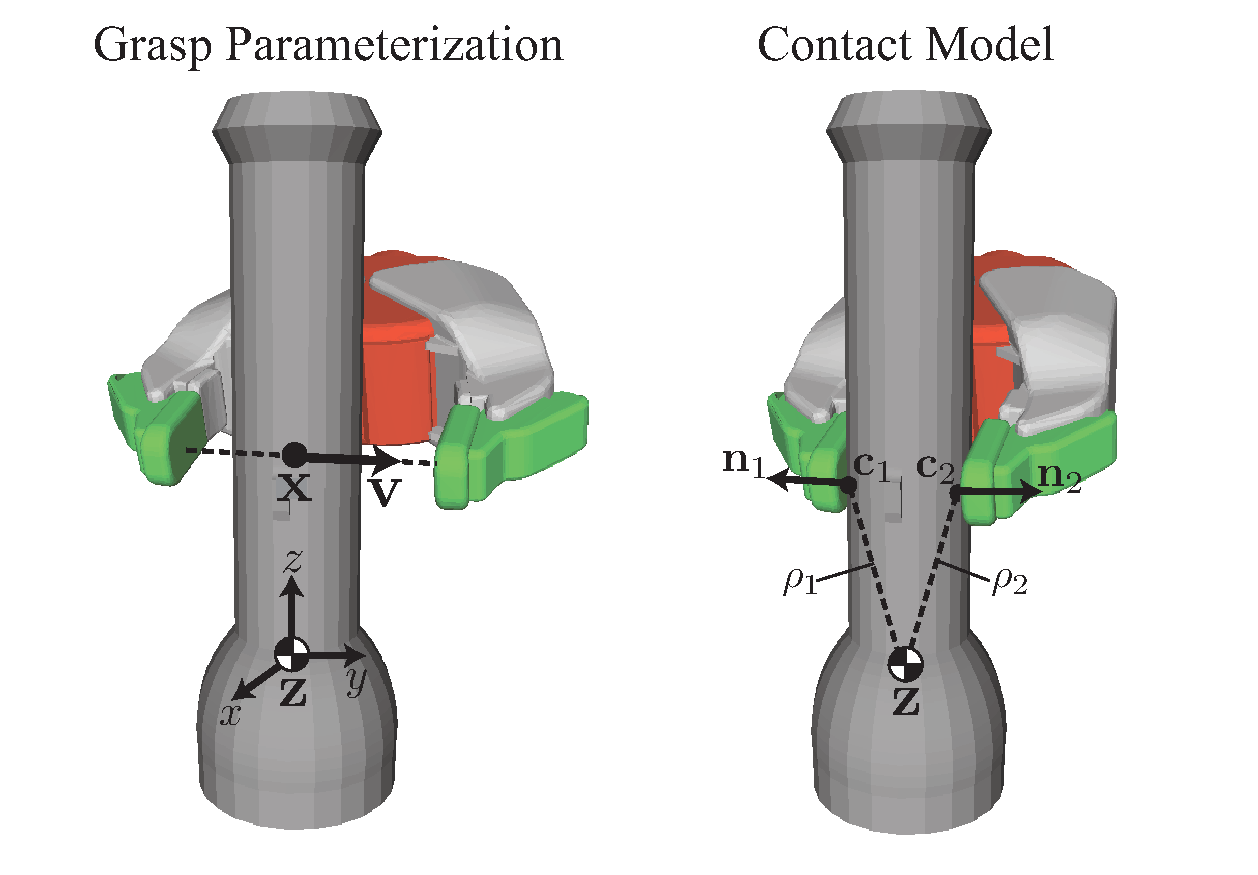
\includegraphics[scale=0.44]{figures/illustrations/dexnet_grasping_model.eps}
\caption{Illustration of grasp parameterization and contact model. (Left) We parameterize parallel-jaw grasps by the centroid of the jaws $\bx \in \mathbb{R}^3$ and approach direction, or direction along which the jaws close, $\bv \in \bS^2$. The parameters $\bx$ and $\bv$ are specified with respect to a coordinate frame at the object center of mass $\bz$ and oriented along the principal directions of the object. (Right) The jaws are closed until contacting the object surface at locations $\bc_1, \bc_2 \in \mathbb{R}^3$, at which the surface has normals $\bn_1, \bn_2 \in \bS^2$. The contacts are used to compute the moment arms $\rho_i = \bc_i - \bz$.
% and $\rho_2  = \bc_2 - \bz$.
}
\figlabel{grasp-model}
\vspace*{-15pt}
\end{figure}

\subsection{Sources of Uncertainty}
\seclabel{uncertainty}
We assume Gaussian distributions on object pose, gripper pose, and friction coefficient to model errors in registration, robot calibration, or classification material properties, respectively. 
We denote by $\mN(\mu,\Sigma)$ a Gaussian distribution with mean $\mu$ and variance $\Sigma$.
Let $\upsilon \sim \mN\left(\mathbf{0}, \Sigma_{\upsilon}\right)$ denote a zero-mean Gaussian on $\bR^6$ and $\mu_{\xi} \in SE(3)$ be a mean object pose.
We define the object pose random variable $\xi = \exp\left( \upsilon^{\wedge} \right) \mu_{\xi}$, where the $\wedge$ operator maps from $\bR^6$ to the Lie algebra $\mathfrak{se}(3)$.
Let $\nu \sim \mN\left(\mu_{\nu}, \Sigma_{\nu}\right)$ denote a Gaussian distribution on gripper pose with mean $\mu_{\nu} \in \mG$.
Let $\gamma \sim \mN\left(\mu_{\gamma}, \Sigma_{\gamma} \right)$ denote a Gaussian distribution on friction coefficient with mean $\mu_{\gamma} \in \mathbb{R}$.
We denote by $\hat{\xi}, \hat{\nu},$ and $\hat{\gamma}$ samples of the random variables. 

\subsection{Contact Model}
\seclabel{contact}
Given a grasp $\bg$ on an object $\mO$ and samples $\hat{\xi}, \hat{\nu},$ and $\hat{\gamma}$, let $\bc_i \in \mathbb{R}^3$ for $i \in {1, 2}$ denote the 3D contact location between the $i$-th gripper jaw and surface as shown in \figref{grasp-model}.
Each contact $\bc_i = \bx + (-1)^{i} (w / 2 - t_i^*) \bv$ where~\cite{mahler2015gp}:
%\vspace{-1ex}
\begin{align*}
	t_i^* &= \myargmin{t \geq 0} t \text{ such that } f\left(\bx +  (-1)^{i} (w / 2 - t) \bv\right) = 0.
\end{align*}
\noindent Let $\bn_i = \nabla f(\bc_i) / \| \nabla f(\bc_i) \|_2$ denote the surface normal at contact $\bc_i$ with tangent vectors $\bt_{i,1}, \bt_{i,2} \in \bS^2$.
To compute the forces that each contact can apply to the object for friction coefficient $\hat{\gamma}$, we discretize the friction cone at $\bc_i$~\cite{pokorny2013c} into a set of $l$ facets with vertices $\mF_{i} = \left\{ \bn_i + \hat{\gamma} \cos \left( \frac{2 \pi j}{l} \right) \bt_{i,1} + \hat{\gamma} \sin \left( \frac{2 \pi j}{l} \right) \bt_{i,2} \big| j = 1, ..., l \right\}$.
Each force $\bbf_{i,j} \in \mF_{i}$ can exert a corresponding torque $\tau_{i,j} = \bbf_{i,j} \times \rho_i$ where $\rho_i = (\bc_i - \bz)$ is the moment arm at $\bc_i$.
Under the soft contact model, each contact $\bc_i$ exerts an additional wrench $\bw_{i,l+1} = (\mathbf{0}, \bn_i)$~\cite{zheng2005}.
Thus the set of all contact wrenches that can be applied by a grasp $\bg$ under the model is $\mW = \{ \bw_{i,j} = (\bbf_{i,j}, \tau_{i,j}) \big| i = 1, 2 \text{ and } j = 1, ..., l+1\}$.

\subsection{Quality Metric}
\seclabel{quality}
In this work we use the probability of force closure ($P_F$), or the ability to resist external force and torques in arbitrary directions~\cite{mahler2015gp}, as the quality metric.
$P_F$ has shown promise in physical experiments~\cite{kim2012physically, weisz2012pose} and is relatively inexpensive to evaluate, allowing us to better study the effects of large amounts of data.

Let $F \in \{0, 1\}$ denote the occurrence of force closure.
Then for a grasp $\bg$ on object $\mO$, $P_F(\bg, \mO) = \mathbb{P}\left(F = 1 \mid \bg, \mO, \xi, \nu, \gamma \right)$.
To compute force closure for a grasp $\bg \in \mG$ on object $\mO \in \mH$ given samples of object pose $\hat{\xi}$, gripper pose $\hat{\nu}$, and friction coefficient $\hat{\gamma}$, we first compute the set of possible contact wrenches $\mW$.
Then $F = 1$ if $\mathbf{0} \in Conv(\mW)$, where $Conv(\cdot)$ denotes the convex hull~\cite{weisz2012pose}.

\subsection{Objective}
We are interested in finding a grasp $\bg^*$ that maximizes $P_F(\bg)$~\cite{kim2012physically, laskey2015bandits, mahler2015gp, weisz2012pose} over a budgeted maximum number of samples $T$.
To perform this as quickly as possible we maximize over the sum of the $P_F$ for all sampled grasps~\cite{laskey2015bandits, srinivas10gaussian}.
As the maximization over the continuous space $\mG$ is computationally expensive, past work has solved this objective by evaluating a discrete set of $K$ candidate grasps $\Gamma = \left\{ \bg_1, ..., \bg_K \right\}$ with Monte-Carlo integration~\cite{kehoe2012toward, weisz2012pose} or Multi-Armed Bandits (MAB) ~\cite{laskey2015bandits}.
In this work, we extend the 2D MAB model of~\cite{laskey2015bandits} to leverage similarities between grasps and prior 3D objects in Dex-Net to reduce the number of samples~\cite{hoffman2013exploiting, pandey2007multi}.